\chapter{Forces and Motion}


\section{Force, Mass, and Acceleration}
A force\index{force} is a push or a pull. Kick a ball, and your foot pushes it. Hold a dog's leash, and the leash pulls your hand. Forces are \textit{vectors}: each has a size and a direction, and we can add them up, even when they point opposite ways. Newton's three laws of motion tell us how forces change the way things move.

\subsection{Newton's First Law}
Newton's First Law of Motion states that an object at rest will stay at rest, and an object in motion will stay in motion with a constant velocity (same speed and direction) unless acted upon by a \emph{net external force}. This means that if there is no net force on an object, it will not \emph{accelerate}. \index{Newton's First Law}

For example, a car that stops pressing the gas on a flat road will eventually stop due to friction, which is a force that acts opposite to the direction of motion. If there were no friction, the car would continue moving at a constant speed forever.

This law is sometimes also referred to as the law of \emph{inertia}, which is the tendency of objects to resist changes in their motion. \index{inertia}
\subsection{Mass, Acceleration, and Newton's Second Law}

Each atom has a \index{mass}mass, which means everything made up of those atoms has mass as 
well (and that is pretty much everything!). We measure mass in grams. A paper clip is about 1 gram of steel. An adult human can have a mass of 70,000 grams, so for larger things, we often talk about kilograms, which is 1000 grams.

The first interesting thing about mass is that objects with more mass
require more force to accelerate. For example, pushing a bicycle so
that it accelerates from a standstill to jogging speed in 2 seconds
requires much less force than pushing a train so that it accelerates
at the same rate.


\index{Newton's Second Law of Motion}
\begin{mdframed}[style=important, frametitle={Newton's Second Law of Motion}]

The force necessary to accelerate an object of mass $m$ at an acceleration of
$a$ is given by:
$$F = m a$$

This is said as ``the force is equal to the mass times the acceleration.''

\end{mdframed}

This is Newton's Second Law of Motion. It may be the most useful equation in all of physics.

What are the units here? We already know that mass is measured in
kilograms. We can measure velocity in meters per second, but that is
different from acceleration. So if we want to go from 0 to 5 meters per second (that is
jogging speed) in two seconds, that is a change in velocity of 2.5
meters per second every second. We would say this acceleration is $2.5
m/s^2$.

\subsubsection{Velocity versus Acceleration}
\index{acceleration}Acceleration is the change in velocity. If an object is speeding up or slowing 
down, it is accelerating. In everyday language, we often use \textit{decelerate} 
to indicate slowing down, but in physics you can use the word accelerate (slowing 
down is just negative acceleration). Since velocity is a vector (it has a 
magnitude and direction), changing direction is \textit{also acceleration}. On 
the other hand, an object moving at a constant velocity (same speed, same 
direction) is \textit{not accelerating}!

\begin{Exercise}[title = {Is it accelerating?}, label = accel]
State whether the described object is accelerating or not. 
\begin{enumerate}
\item A satellite orbiting the Earth at a constant speed.
\item A car moving due west at a constant 30 mile per hour.
\item A child coming to a stop on their bicycle.
\item A roller coaster going around a loop at a constant speed.
\item A roller coaster speeding up as it goes down the initial hill.
\item A book sitting on a table. 
\end{enumerate}
\end{Exercise}

\begin{Answer}[ref = accel]
\begin{enumerate}
\item Acceleration: the satellite is moving in a circle, therefore changing 
direction and accelerating.
\item Not acceleration: the car is not changing speed or direction.
\item Acceleration: the child is changing speed.
\item Acceleration: the roller coaster is changing direction.
\item Acceleration: the roller coaster is changing speed. 
\item Not acceleration: the book is not changing speed or direction.
\end{enumerate}
\end{Answer}

It is a common misconception that all objects in motion are accelerating. If an 
object is moving with a constant velocity (same speed, same direction), then it 
is not accelerating. 

\subsubsection{Calculating Acceleration}
When an object is speeding up or slowing down, we can calculate the acceleration 
by dividing the change in velocity by the time it takes to make that change. 

\begin{mdframed}[style = important, frametitle = {Calculating Acceleration}]
The acceleration of an object from an initial velocity, $v_i$, to a final
velocity, $v_f$, over a period of time, $t$, is given by:

$$a = \frac{v_f - v_i}{t}$$
\end{mdframed}

Notice that if the velocity does not change, then $v_f - v_i = 0$ and the 
acceleration is also zero.

\textbf{Example}: Your car can go from zero to 60 mph in 3 seconds. What is the
acceleration in $m / s^2$?

\textbf{Solution}: First, let us convert from the imperial units of miles per
hour to the SI units of meters per second. You can do this using a search engine, 
but we will show how to do it by hand below. (You will learn more about this 
method in the Units chapter).

$$\frac{60 \text{ miles}}{1 \text{ hour}} \cdot \frac{1.61 \text{ km}}{1 
\text{ mile}} \cdot \frac{1000\text{ m}}{1\text{ km}} \cdot \frac{1\text{ hour}}{
3600\text{ seconds}} \approx \frac{26.82\text{ m}}{s}$$

Now we have the starting velocity (0 m/s), the ending velocity (26.82 m/s), and 
the time (3 s), and we can find the acceleration:
$$a = \frac{v_f - v_i}{t} = \frac{26.82\frac{m}{s} - 0\frac{m}{s}}{3s} \approx 
8.94 \frac{m}{s^2}$$

\subsubsection{Determining Force}
What about measuring force? The unit is named after Newton\index{newton (unit)}: the
force needed to accelerate one kilogram at $1 m/s^2$ is \textit{one
newton}, written N. An apple sitting in your hand pushes down with about one newton.

$$1 N = 1 \frac{kg \cdot m}{s^2}$$

\textbf{Example}: If the car in the above example has a mass of 1500 kg, how much 
force does the engine use to accelerate the car?

\textbf{Solution}: We have already found the car's acceleration: 8.94 $m/s^2$. 
With the mass and acceleration, we can use Newton's Second Law to find the force 
needed to accelerate the car:
$$F = m \cdot a = 1500\text{ kg} \cdot 8.94 \frac{m}{s^2} = 13410\text{ N}$$

\begin{Exercise}[title={Acceleration}, label=acceleration_train]

While driving a bulldozer, you come across a train car (with no brakes
and no locomotive) sitting on a track in the middle of a city. The train car
has a label telling you that it has a mass of 2,400 kg. There is a time-bomb
welded to the interior of the train car, and the timer tells you that
you can safely push the train car for 120 seconds. To get the train
car to where it can explode safely, you need to accelerate it to 20 meters per
second. Fortunately, the track is level and the train car's wheels have
almost no rolling resistance.

With what force, in newtons, do you need to push the train for those 120 seconds?

\end{Exercise}
\begin{Answer}[ref=acceleration_train]
If you accelerate to 20 m/s in 120 s, the acceleration is:
$$a = \frac{v_f - v_i}{t} = \frac{20\text{ m/s} - 0\text{ m/s}}{120\text{ s}} = 
\frac{1}{6} \frac{m}{s^2}$$

To achieve this acceleration, you will need to apply a force of:
$$F = m \cdot a = 2400\text{ kg} \cdot \frac{1}{6} \frac{m}{s^2} = 400\text{ }N$$
\end{Answer}

\subsection{Net Force}
So far, we have looked at examples where only one force is acting on an object. In 
reality, there are usually multiple forces acting on an object. For example, the 
engine pushes your car forward while friction pulls it backwards. Or your chair 
is pushing up on you while gravity pulls you down. How then can we describe the 
motion of an object if more than one force is acting on it?

We can rearrange Newton's Law:
$$a = \frac{F_{net}}{m}$$

This means that an object's acceleration is directly proportional to the 
\textit{net force} acting on the object and inversely proportional to the object's 
mass. The \textit{net force} is the vector sum of all the forces acting on an 
object\index{net force}. The vector sum just means we have to take the direction of 
the force into account. Usually, up and right are positive while down and left are 
negative. You can see some examples in figure \ref{fig:net_forces}.

\begin{figure}
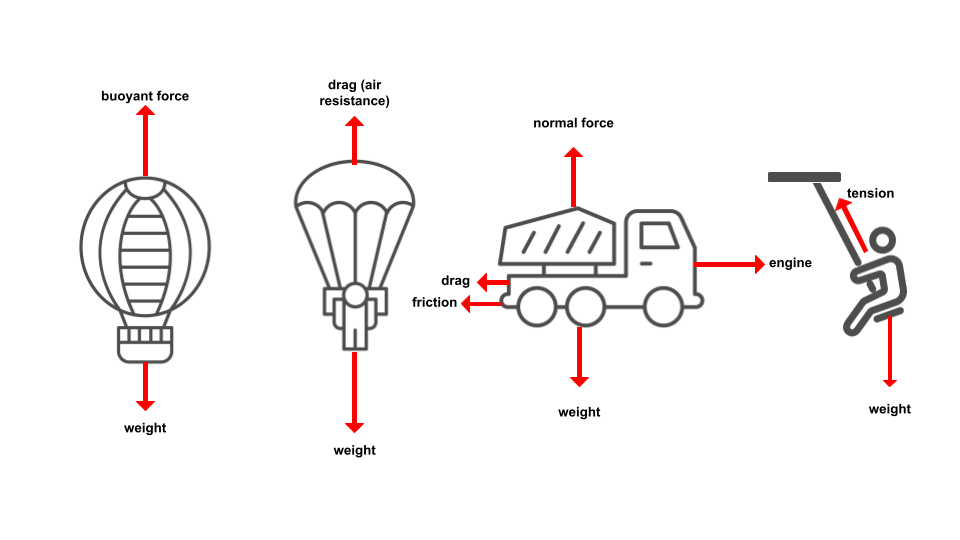
\includegraphics[width=6in]{net_forces.png}
\caption{The hot air balloon has an upwards net force. The parachuter has a 
downwards net force. The truck has a rightward net force. The swinger has a 
leftward net force.}
\label{fig:net_forces}
\end{figure}

For now, we will only look at parallel forces (up/down or left/right). You will learn 
to use vector addition to combine orthogonal (at right angles) and skew (at angles
other than parallel or right) forces in a later chapter. 

\textbf{Example}: A donkey and a horse are each pulling a cart. The donkey pulls 
to the left with a force of 1500 N, while the horse pulls to the right with a 
force of 2000 N. What is the net force on the cart? If the cart has a mass of 
1000 kg, in what direction and with what magnitude will the cart accelerate?

\textbf{Solution}: We begin by drawing a diagram (this is good practice - while 
a diagram may not be necessary for such a simple question, it will be very useful 
as we examine more complex scenarios in future chapters). 

\begin{center}
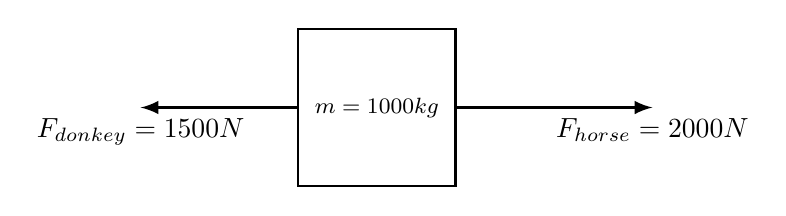
\begin{tikzpicture}
    \draw[thick, black] (-1, -1) rectangle (1,1);
    \draw[very thick, black, -latex] (-1, 0) -- (-3, 0) node[below] {$F_{donkey} 
    = 1500N$};
    \draw[very thick, black, -latex] (1, 0) -- (3.5, 0) node[below] {$F_{horse}=
    2000N$};
    \node[font = \footnotesize] at (0,0) {$m=1000kg$};
\end{tikzpicture}
\end{center}

It is customary to take right as positive, so the horse applies a positive force 
while the donkey applies a negative force to the cart. Therefore, the net force 
is:

$$F_{net} = F_{horse} - F_{donkey} = 2000N - 1500N = 500N$$

Since the net force is positive, it points to the right and the cart will 
accelerate to the right at a rate of:
$$a = \frac{F_{net}}{m} = \frac{500 N}{1000 kg} = 0.5 \frac{m}{s^2}$$

\begin{Exercise}[title = {Net Force and Acceleration}, label = netF]
Rank the acceleration of the boxes shown below from greatest to least. All 
surfaces are frictionless and each box starts at rest. Take left as negative, and 
negative accelerations are less than a zero acceleration.

\begin{tikzpicture}
    \draw[thick, fill=gray!50] (-1.5, 1.5) rectangle (-0.5, 2) node[above, 
    xshift = -0.5cm] {\textbf{A}};
    \node[font = \footnotesize] at (-1, 1.75) {1 kg};
    \draw[pattern = north west lines] (-2, 1.5) rectangle (0, 1.25);
    \draw[very thick, -latex] (-0.5, 1.75) -- (0.5, 1.75) node[above] 
    {$F_1 = 4N$};
    \draw[very thick, -latex] (-1.5, 1.75) -- (-2.25, 1.75) node[above] 
    {$F_2 = 3N$};

    \draw[thick, fill=gray!50] (4, 1.5) rectangle (5, 2) node[above, 
    xshift=-0.5cm] {\textbf{B}};
    \node[font = \footnotesize] at (4.5, 1.75) {1 kg};
    \draw[pattern = north west lines] (3.5, 1.5) rectangle (5.5, 1.25);
    \draw[very thick, -latex] (4, 1.75) -- (3, 1.75) node[above] 
    {$F_2 = 4N$};
    \draw[very thick, -latex] (5, 1.75) -- (5.75, 1.75) node[above] 
    {$F_1 = 3N$};

    \draw[thick, fill=gray!50] (-1.5, -0.5) rectangle (-0.5, 0) node[above, 
    xshift=-0.5cm] {\textbf{C}};
    \node[font = \footnotesize] at (-1, -0.25) {0.5 kg};
    \draw[pattern = north west lines] (-2, -0.5) rectangle (0, -0.75);
    \draw[very thick, -latex] (-0.5, -0.25) -- (0.5, -0.25) node[above] 
    {$F_1 = 4N$};
    \draw[very thick, -latex] (-1.5, -0.25) -- (-2.25, -0.25) node[above] 
    {$F_2 = 3N$};

    \draw[thick, fill=gray!50] (4, -0.5) rectangle (5, 0) node[above, 
    xshift=-0.5cm] {\textbf{D}};
    \node[font = \footnotesize] at (4.5, -0.25) {0.5 kg};
    \draw[pattern = north west lines] (3.5, -0.5) rectangle (5.5, -0.75);
    \draw[very thick, -latex] (4, -0.25) -- (3, -0.25) node[above] {$F_2 = 4N$};
    \draw[very thick, -latex] (5, -0.25) -- (5.75, -0.25) node[above] 
    {$F_1 = 3N$};

    \draw[thick, fill=gray!50] (-1.5, -2.5) rectangle (-0.5, -2) node[above, 
    xshift=-0.5cm] {\textbf{E}};
    \node[font = \footnotesize] at (-1, -2.25) {0.5 kg};
    \draw[pattern = north west lines] (-2, -2.5) rectangle (0, -2.75);
    \draw[very thick, -latex] (-0.5, -2.25) -- (0.75, -2.25) node[above] 
    {$F_1 = 5N$};
    \draw[very thick, -latex] (-1.5, -2.25) -- (-2.75, -2.25) node[above] 
    {$F_2 = 5N$};    

    \draw[thick, fill=gray!50] (4, -2.5) rectangle (5, -2) node[above, 
    xshift=-0.5cm] {\textbf{F}};
    \node[font = \footnotesize] at (4.5, -2.25) {1 kg};
    \draw[pattern = north west lines] (3.5, -2.5) rectangle (5.5, -2.75);
    \draw[very thick, -latex] (4, -2.25) -- (2.75, -2.25) node[above] 
    {$F_2 = 5N$};
    \draw[very thick, -latex] (5, -2.25) -- (6.25, -2.25) node[above] 
    {$F_1 = 5N$};
\end{tikzpicture}
\end{Exercise}

\begin{Answer}[ref = netF]
C, A, E/F, B, D
$$a_A = \frac{F_{net, A}}{m_A} = \frac{4N - 3N}{1kg} = \frac{1N}{1kg} = 1 
\frac{m}{s^2}$$
$$a_B = \frac{F_{net, B}}{m_B} = \frac{3N - 4N}{1kg} = \frac{-1N}{1kg} = -1 
\frac{m}{s^2}$$
$$a_C = \frac{F_{net, C}}{m_C} = \frac{4N - 3N}{0.5kg} = \frac{1N}{0.5kg} = 2 
\frac{m}{s^2}$$
$$a_D = \frac{F_{net, D}}{m_D} = \frac{3N - 4N}{0.5kg} = \frac{-1N}{0.5kg} = -2 
\frac{m}{s^2}$$
$$a_E = \frac{F_{net, E}}{m_E} = \frac{5N - 5N}{0.5kg} = \frac{0N}{0.5kg} = 0 
\frac{m}{s^2}$$
$$a_F = \frac{F_{net, F}}{m_F} = \frac{5N - 5N}{1kg} = \frac{0N}{1kg} = 0 
\frac{m}{s^2}$$
\end{Answer}

\subsection{Normal Force and Apparent Weight}
If you were to stand on a scale while riding an elevator, you would see the scale 
fluctuate as the elevator accelerates up and down (if you have a bathroom scale 
and live in a building with an elevator, you can try this yourself!). The reading 
on the scale is your \textit{apparent weight}\index{apparent weight} and is equal to the normal force 
between you and the floor. 

What is a \textit{normal force}\index{normal force}? First, the word ``normal" does not have the 
colloquial meaning of average or usual. In mathematics, ``normal" means 
perpendicular. A normal force is perpendicular to the \emph{contact} surface between 
two objects. Let us look at a person standing at rest. We know that gravity is 
pulling down on the person:

\begin{center}
    \begin{tikzpicture}
        %\draw[step=1cm, gray, very thin] (-2, -4) grid (2, 0);

        %floor
        \draw[pattern = north west lines] (-4, 0) rectangle (4, -0.5);

        %arrows and labels
        \draw[red, fill=red] (0, -2) -- (0.5, -1.5) -- (0.25, -1.5) -- (0.25, 0.5) -- 
        (-0.25, 0.5) -- (-0.25, -1.5) -- (-0.5, -1.5) -- cycle;
        \node[] at (0, -2.25) {Weight};
        \node[] at (0, -2.75) {$F_g = mg$};
    
        %person fill
        \draw[gray, fill=gray] (-0.5, 0.5) circle (0.5cm);
        \draw[gray, fill=gray] (0.5, 0.5) circle (0.5cm);
        \draw[gray, fill=gray] (-1, 0.5) rectangle (1, 4);
        \draw[gray, fill=gray] (-1.25, 2.5) circle (0.25cm);
        \draw[gray, fill=gray] (1.25, 2.5) circle (0.25cm);
        \draw[gray, fill=gray] (-1.5, 2.5) rectangle (-1, 5);
        \draw[gray, fill=gray] (1, 2.5) rectangle (1.5, 5);
        \draw[gray, fill=gray] (0, 6.25) circle (0.75cm);
        \draw[gray, fill=gray] (-1, 5) circle (0.5cm);
        \draw[gray, fill=gray] (1, 5) circle (0.5cm);
        \draw[gray, fill=gray] (-1, 4) rectangle (1, 5.5);

        %person outline
        \draw[] (-1, 4.5) -- (-1, 0.5) arc (180:360:0.5);
        \draw[] (0, 0.5) arc (180:360:0.5) -- (1,4.5);
        \draw[] (0, 0.5) -- (0,2.75);
        \draw[] (1, 2.5) arc (180:360:0.25) -- (1.5, 5) arc (0:90:.5) -- 
        (-1, 5.5) arc (90:180:0.5) -- (-1.5, 2.5) arc (180:360:0.25);
        \draw[] (0, 6.25) circle (0.75cm);
    \end{tikzpicture}
\end{center}

Since the person is not accelerating, there must be some other force acting on 
them in the upwards direction that balances out the person's weight (recall that 
if $a=0 m/s^2$, then it must be true that $F_{net} = 0N$). In this case, the 
balancing force is the \textit{normal force} of the floor pushing up on the 
person's feet:

\begin{center}
    \begin{tikzpicture}
        %\draw[step=1cm, gray, very thin] (-2, -4) grid (2, 0);

        %floor
        \draw[pattern = north west lines] (-4, 0) rectangle (4, -0.5);

        %down arrows and labels
        \draw[red, fill=red] (-0.5, -2) -- (0, -1.5) -- (-0.25, -1.5) -- 
        (-0.25, 0.5) -- (-0.75, 0.5) -- (-0.75, -1.5) -- (-1, -1.5) -- cycle;
        \node[] at (-0.5, -2.25) {Weight};
        \node[] at (-0.5, -2.75) {$F_g = mg$};
    
        %person fill
        \draw[gray, fill=gray] (-0.5, 0.5) circle (0.5cm);
        \draw[gray, fill=gray] (0.5, 0.5) circle (0.5cm);
        \draw[gray, fill=gray] (-1, 0.5) rectangle (1, 4);
        \draw[gray, fill=gray] (-1.25, 2.5) circle (0.25cm);
        \draw[gray, fill=gray] (1.25, 2.5) circle (0.25cm);
        \draw[gray, fill=gray] (-1.5, 2.5) rectangle (-1, 5);
        \draw[gray, fill=gray] (1, 2.5) rectangle (1.5, 5);
        \draw[gray, fill=gray] (0, 6.25) circle (0.75cm);
        \draw[gray, fill=gray] (-1, 5) circle (0.5cm);
        \draw[gray, fill=gray] (1, 5) circle (0.5cm);
        \draw[gray, fill=gray] (-1, 4) rectangle (1, 5.5);

        %person outline
        \draw[] (-1, 4.5) -- (-1, 0.5) arc (180:360:0.5);
        \draw[] (0, 0.5) arc (180:360:0.5) -- (1,4.5);
        \draw[] (0, 0.5) -- (0,2.75);
        \draw[] (1, 2.5) arc (180:360:0.25) -- (1.5, 5) arc (0:90:.5) -- 
        (-1, 5.5) arc (90:180:0.5) -- (-1.5, 2.5) arc (180:360:0.25);
        \draw[] (0, 6.25) circle (0.75cm);

        %up arrows and labels
         \draw[blue, fill=blue] (0.25, 0) -- (0.25, 1.5) -- (0, 1.5) -- 
         (0.5, 2) -- (1, 1.5) -- (0.75, 1.5) -- (0.75, 0) -- cycle;
         \node[] at (0.5, 2.25) {$F_N$};
         \node[] at (0.5, 2.75) {Normal Force};
    \end{tikzpicture}
\end{center}

%fix me explanation of normal force? intuitive explanation of deformation, atoms being pressed together and repelling, rebound of table. There's a demo where you shine a laser at an angle on a mirror flat on a table, then put weight on the table. students can see that the table deforms and helps students to "justify" where the normal force comes from. didn't find a good youtube video but i'll keep looking

When you step on a bathroom scale, it is actually measuring the normal force! 
When you are not accelerating, your weight and the normal force between you and 
the scale are equal, so the scale gives you an accurate measure of your weight. 
Let us look at what happens if you are accelerating, as in an elevator.

\textbf{Example}: Maria has a mass of 80. kg. If the elevator in her apartment 
building initially accelerates at 0.50 $m/s^2$, what is her apparent weight as 
the elevator begins to move down?

\textbf{Solution}: We begin with a diagram:
\begin{center}
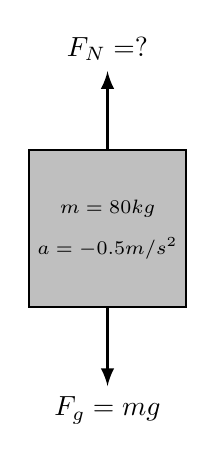
\begin{tikzpicture}
	\draw[thick, fill = gray!50] (-1, -1) rectangle (1, 1);
	\node[font = \scriptsize] at (0,0.25) {$m=80kg$};
	\node[font = \scriptsize] at (0, -0.25) {$a=-0.5m/s^2$};
	\draw[very thick, -latex] (0, -1) -- (0, -2) node[below] {$F_g = mg$};
	\draw[very thick, -latex] (0, 1) -- (0, 2) node[above] {$F_N = ?$};
\end{tikzpicture}
\end{center}

Her apparent weight is the normal force. Seeing that the net force acting on 
Maria is given by $F_N - F_g$, we can use Newton's Second Law to find $F_N$:

$$F_{net} = F_N - F_g = ma$$
$$F_N - \left( 80 kg \right) \left(9.8 \frac{m}{s^2} \right) = \left( 80 kg 
\right) \left( -0.5 \frac{m}{s^2} \right)$$
$$F_N = \left( 80 kg \right) \left( 9.8 \frac{m}{s^2} - 0.5 \frac{m}{s^2} 
\right) = 744 N$$

Maria's apparent weight is 744 newtons when the elevator is accelerating 
downwards. 

\begin{Exercise}[title = Moving Elevators, label = elevator]
A 700-N person is standing on a scale in an elevator. Rank the reading on the 
scale from greatest to least for the following scenarios:
\begin{enumerate}
\item The elevator has an initial upward velocity of 2 m/s and an upward 
acceleration of 3 $m/s^2$
\item The elevator is initially at rest and has an upward acceleration of 3 
$m/s^2$
\item The elevator has an initial downward velocity of 2 m/s and an upward 
acceleration of 5 $m/s^2$
\item The elevator is initially at rest and has a downward acceleration of 
9.8 $m/s^2$
\item The elevator has an initial upward velocity of 2 m/s and a downward 
acceleration of 5 $m/s^2$
\item The elevator has an initial downward velocity of 2 m/s and is not 
accelerating 
\end{enumerate}
\end{Exercise}

\begin{Answer}[ref = elevator]
3, 1/2, 6, 5, 4
The velocity does not affect the apparent weight, only the acceleration. If the 
elevator is accelerating upwards, the apparent weight increases. If the elevator 
is accelerating downwards, the apparent weight decreases. In fact, for scenario 
4, the elevator is in free-fall and the person has no apparent weight. When the 
elevator is not accelerating, the person's apparent weight is their true weight. 
\end{Answer}

On flat ground, for an object that is not accelerating up or down, the normal force is equal in size to the object's weight. The normal force also controls another contact force, friction, which you will meet later in this chapter. On a ramp, the normal force points \emph{perpendicular} to the ramp, not straight up.

\subsection{Newtons and Joules}
Energy is measured in joules. Compare the units of a newton and a joule:
$$N = \frac{kg \cdot m}{s^2} \qquad J = \frac{kg \cdot m^2}{s^2} = N \cdot m$$

A joule is a newton times a meter. That is a hint: push with a force (newtons) through a distance (meters), and you change an object's energy (joules). This idea, the work-energy theorem, comes in a later chapter. 

\subsection{Newton's Third Law}
%FIXME expand
Newton's Third Law says that every action has an equal and opposite reaction. \index{Newton's Third Law}
In other words, if body \(A\) exerts a force on body \(B\), then body \(B\) simultaneously 
exerts a force of equal magnitude and opposite direction on body \(A\).
Mathematically, we can express this as:
\[
    \mathbf{F}_{\!AB} \;=\; -\,\mathbf{F}_{\!BA}
\]
Forces always come in pairs. If box 1 pushes on box 2, then box 2 pushes back on box 1 just as hard, no matter which box is heavier: $F_{\text{Box 1 on 2}} = -F_{\text{Box 2 on 1}}$.
You will see these pairs everywhere: air pushing back on a moving car, coupled train cars tugging on each other, and planets pulling on each other. 

Note the following:
\begin{itemize}
    \item Action-reaction pairs do \emph{not} cancel when applying Newton's Second Law to a single body.
    \item The forces are always of the same type (both contact, both gravitational, etc).
    \item They occur simultaneously; there is no time delay.
\end{itemize}

Watch out for a classic mistake: a book's weight and the normal force on it are \emph{not} an action-reaction pair, even though they are often equal and opposite. Both act on the book, and they are different types of force. The partner of the Earth pulling down on the book is the book pulling up on the Earth. The partner of the table pushing up on the book is the book pushing down on the table.
\textbf{Example:}
Consider a swimmer pushing the wall of a pool. What forces are in play?

\textbf{Solution:}
While the swimmer exerts a force \(\mathbf{F}_{\text{wall}}\) on the wall, the wall exerts the reaction \(-\mathbf{F}_{\text{wall}}\) on the swimmer, propelling the swimmer forward.  
Although the wall does not move due to mass and acceleration differences, the forces are equal and opposite. 


\section{Free Body Diagrams}
Now that you have mastered modeling \textit{how things move}, you can learn to 
model \textit{why things move}. Recall Newton's Second Law:
$$F = ma$$

This is a simplification: what Newton's Second Law says in total is "the 
acceleration of a body is directly proportional to the \textit{net force} 
acting on the body and inversely proportional to the mass of the body." 
Mathematically, that would be:
$$a = \frac{\Sigma F}{m}$$

Where $\Sigma F$ is the vector sum of all the individual forces acting on the 
body. This sum is also called the \textit{net force}. To visualize the magnitude 
and direction of the net force, it can be very helpful to draw a \index{free body diagram}free body
diagram. 

\subsection{Interpreting Free Body Diagrams}
Before you learn to draw your own free body diagrams (FBDs), let us examine and 
analyze a few. Here is a FBD for an accelerating car:

\begin{center}
    \begin{tikzpicture}
        \draw[thick] (-1, -1) rectangle (1, 1);
        \draw[fill=black] (0,0) circle (0.4mm);
        \draw[-latex] (0, 0) -- (0, -3) node[below] {$F_g$};
        \draw[-latex] (0,0) -- (-1.25, 0) node[left] {$F_f$};
        \draw[-latex] (0,0) -- (0, 3) node[above] {$F_N$};
        \draw[-latex] (0,0) -- (2, 0) node[right] {$F_{engine}$};
        
    \end{tikzpicture}
\end{center}

We can consider the $x$ and $y$ axes separately. On the $y$-axis, we see that 
the weight ($F_g$) is the same magnitude as the normal force ($F_N$) because the arrows are the same length. This 
means in the $y$ direction, the forces are balanced, and thus we do not expect 
to see acceleration in the $y$ direction. This makes intuitive sense: if you are 
accelerating your car on a flat road, your car does not go up into the air. How 
about the $x$ direction? Here we see friction ($F_f$) pulling the car backwards 
while the engine is pushing the car forwards. In this case, the forces are 
\textit{not} balanced. See how the $F_{engine}$ arrow is longer than the $F_f$ 
arrow? This means the forward force from the engine is \textit{greater in magnitude}
than the backward force of $F_f$. Therefore, the \textit{net force} in the $x$ 
direction is to the right, and the car will accelerate to the right. 

%Here's a more complicated example, where not all the forces are perpendicular to 
%each other. Consider a child sledding down a hill:
%\begin{center}
% FIXME: Commit images.
%\includegraphics[width=5in]{sledder.png}
%\end{center}

\subsection{Drawing Free Body Diagrams}

A free body diagram consists of the object, usually represented as a simple 
square, with various arrows representing the forces acting on the object. The 
direction and relative lengths of the arrows show the direction and relative 
strength of the forces. Here is a free body diagram for a 2-kg hammer in free fall 
through the air on Earth:

\begin{center}
    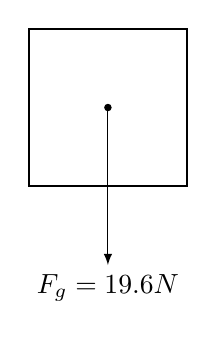
\begin{tikzpicture}
        \draw[thick] (-1, -1) rectangle (1, 1);
        \draw[fill=black] (0,0) circle (0.4mm);
        \draw[-latex] (0, 0) -- (0, -2) node[below] {$F_g = 19.6N$};
    \end{tikzpicture}
\end{center}

% Both methods are useful; choose the one that you prefer. 

\subsubsection{Objects At Rest}
If an object is at rest, then its acceleration must be $0 \frac{m}{s^2}$. By 
Newton's Second Law, the \textit{net force} acting on that object must also be 
zero. Does this mean there are no forces acting on the object? NO! It means all 
the forces are \index{balanced forces}\textit{balanced}: for every upwards force, there is an equal 
downwards force, and so on. Consider the same 2-kg hammer, but this time it is 
sitting on a table. We know gravity must be acting on the hammer, so let us begin 
with that:

\begin{center}
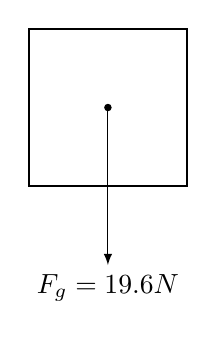
\begin{tikzpicture}
 	\draw[thick] (-1, -1) rectangle (1, 1);
    \draw[fill=black] (0,0) circle (0.4mm);
    \draw[-latex] (0, 0) -- (0, -2) node[below] {$F_g = 19.6N$};
\end{tikzpicture}
\end{center}
% FIXME 
\begin{Exercise}[title = {Blocks on a Table}, label = block1]
[This exercise was originally presented as a free-response question on the 2015 
AP Physics 1 exam.] Two blocks are connected with a string and two pulleys over 
a table, as shown in the figure. Block 1 has a mass of 3 kg and Block 2 has a 
mass of 9 kg. The blocks are released from rest. Treat the string as massless 
and the pulleys as massless and frictionless when answering the questions below. 

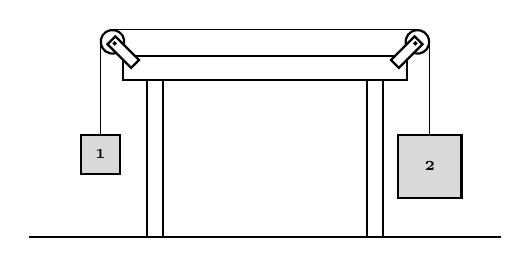
\begin{tikzpicture}
        \draw[thick] (-3, 0) -- (3, 0);
        \draw[thick] (-1.5, 0) rectangle (-1.3, 2);
        \draw[thick] (1.5, 0) rectangle (1.3, 2);
        \draw[thick] (-1.8, 2) rectangle (1.8, 2.3);
        \draw[draw = black, thick, fill=white] (-1.7, 2.15) -- (-1.6, 2.25) -- (-1.9, 2.55) -- (-2, 2.45) -- cycle; 
        \draw[draw=black, thick, fill=white] (1.7, 2.15) -- (1.6, 2.25) -- (1.9, 2.55) -- (2, 2.45) -- cycle;
        \draw[thick, fill=black] (-1.91, 2.46) circle (0.1mm);
        \draw[thick] (-1.79, 2.45) arc (-12:285:0.15);
        \draw[thick, fill=black] (1.91, 2.46) circle (0.1mm);
        \draw[thick] (1.897, 2.335) arc (-105:192:0.15);
        \draw[thin] (-1.94, 2.6382) -- (1.94, 2.6382);
        \draw[thin] (-2.0935, 2.49) -- (-2.0935, 1.3);
        \draw[thin] (2.0927, 2.49) -- (2.0927, 1.3);
        \draw[thick, draw = black, fill = gray!30] (-2.34, 1.3) rectangle (-1.84, 0.8);
        \node[font = \tiny] at (-2.09, 1.05) {\textbf{1}};
        \draw[thick, draw = black, fill = gray!30] (1.69, 1.3) rectangle (2.4954, 0.4946);
        \node[font = \tiny] at (2.0927, 0.8973) {\textbf{2}};
    \end{tikzpicture}
    
\begin{enumerate}
\item Draw free body diagrams for both blocks. Correctly show the relative 
magnitude of the forces using the relative lengths of the vectors. 
\item Before doing any calculations, describe each block's acceleration as (a) 
positive or negative, (b) having a magnitude greater or less than \textit{g}. 
Take the upward direction as positive. 
\item Calculate the acceleration of each block. Take the upward direction as 
positive and express your answer in terms of \textit{g}. 
\end{enumerate}
\end{Exercise}

\begin{Answer}[ref = block1]
\begin{enumerate}
    \item Each block is acted on by gravity and the \index{tension}tension of the string. The 
    force of gravity on block 2 is 3 times that of block 1, and the tension 
    vector should be between the lengths of the gravity vectors:
    \begin{center}
        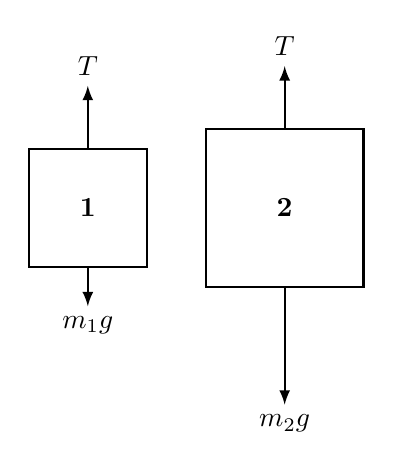
\begin{tikzpicture}
            \draw[thick] (-2, 1) rectangle (-0.5, -0.5);
            \draw[thick] (2.25, 1.25) rectangle (0.25, -0.75);
            \node[] at (-1.25, 0.25) {\textbf{1}};
            \node[] at (1.25, 0.25) {\textbf{2}};
            \draw[thick, -latex] (-1.25, -0.5) -- (-1.25, -1) node[below] {$m_1g$};
            \draw[thick, -latex] (-1.25, 1) -- (-1.25, 1.8) node[above] {$T$};
            \draw[thick, -latex] (1.25, -0.75) -- (1.25, -2.25) node[below] {$m_2g$};
            \draw[thick, -latex] (1.25, 1.25) -- (1.25, 2.05) node[above] {$T$};
        \end{tikzpicture}
    \end{center}

    \item Block 1 will have a positive acceleration and Block 2 a negative one. 
    Both magnitudes are less than \textit{g}: Block 2 falls, but the string 
    holds it back, so it falls more slowly than it would on its own.

    \item Since the blocks are connected, they will move as a \index{system of objects}system and 
    therefore have the same magnitude acceleration. From this, the free body 
    diagrams, and Newton's Second Law, we know that:
    $$m_1 a  = T - m_1 g$$
    $$m_2 \left( - a \right) = T - m_2 g$$

    We know $m_1$ and $m_2$, so the two unknowns are $T$ and $a$. One way to 
    solve this system of equations would be to subtract equation 2 from equation 1:
    $$m_1 a + m_2 a = m_2 g - m_1 g$$
    $$a = \frac{m_2 - m_1}{m_1 + m_2} g$$

    Substituting for the masses, we see that:
    $$a = \frac{9 - 3}{9 + 3}g = \frac{6}{12}g = \frac{1}{2}g$$

    Therefore, Block 1 is accelerating at $+\frac{1}{2}g$ and Block 2 is 
    accelerating at $-\frac{1}{2}g$.
\end{enumerate}
\end{Answer}

Now here is an interesting question: what happens if we add another mass to the 
system? Imagine that a third block with a mass of 15 kg is laid on the table 
from the previous exercise and the string is attached to each side, as shown 
below. 
\begin{center}
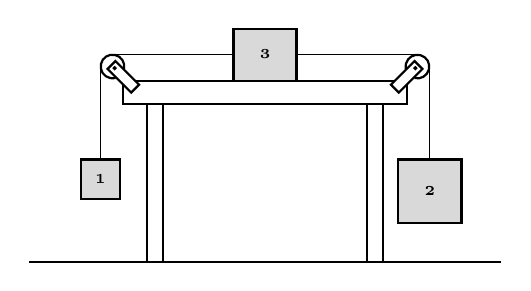
\begin{tikzpicture}
        \draw[thick] (-3, 0) -- (3, 0);
        \draw[thick] (-1.5, 0) rectangle (-1.3, 2);
        \draw[thick] (1.5, 0) rectangle (1.3, 2);
        \draw[thick] (-1.8, 2) rectangle (1.8, 2.3);
        \draw[draw = black, thick, fill=white] (-1.7, 2.15) -- (-1.6, 2.25) -- (-1.9, 2.55) -- (-2, 2.45) -- cycle; 
        \draw[draw=black, thick, fill=white] (1.7, 2.15) -- (1.6, 2.25) -- (1.9, 2.55) -- (2, 2.45) -- cycle;
        \draw[thick, fill=black] (-1.91, 2.46) circle (0.1mm);
        \draw[thick] (-1.79, 2.45) arc (-12:285:0.15);
        \draw[thick, fill=black] (1.91, 2.46) circle (0.1mm);
        \draw[thick] (1.897, 2.335) arc (-105:192:0.15);
        \draw[thin] (-1.94, 2.6382) -- (1.94, 2.6382);
        \draw[thin] (-2.0935, 2.49) -- (-2.0935, 1.3);
        \draw[thin] (2.0927, 2.49) -- (2.0927, 1.3);
        \draw[thick, draw = black, fill = gray!30] (-2.34, 1.3) rectangle (-1.84, 0.8);
        \node[font = \tiny] at (-2.09, 1.05) {\textbf{1}};
        \draw[thick, draw = black, fill = gray!30] (1.69, 1.3) rectangle (2.4954, 0.4946);
        \node[font = \tiny] at (2.0927, 0.8973) {\textbf{2}};
        \draw[thick, draw = black, fill = gray!30] (-0.4, 2.3) rectangle (0.4, 2.96);
        \node[font = \tiny] at (0, 2.638) {\textbf{3}};
    \end{tikzpicture}
\end{center}

We could redraw free body diagrams for all three blocks, noting that the 
tensions on either side of Block 3 will be different. Then, we would have 
another system of equations to solve and we could find the acceleration. Or, 
we could think about the entire system. Originally, the net force on the 
two-block system was 58.8 Newtons (the weight of the larger block minus the 
weight of the smaller block). And the mass of the entire two-block system was 
12 kilograms. We can apply Newton's Second Law:
$$a = \frac{58.8 N}{12 kg} = 4.9 \frac{m}{s^2} = \frac{1}{2}g$$

(Notice, this is the same answer we found in the previous exercise). What 
changes when we add a third, 15-kg block? The net force on the system does not 
change: the table pushes back up on the third block with a force equal to the 
block's weight. However, the total mass of the system has changed: it is 
increased. Now the total mass is 27 kg, and we can again apply Newton's Second 
Law:
$$a = \frac{58.8 N}{27 kg} \approx 2.18 \frac{m}{s^2}$$

This answer makes sense: the mass of the system has increased while the net 
force acting on the system has stayed the same, resulting in a slower acceleration. 

Now, what if instead of blocks resting on level tables, the blocks were on an incline? Ramps need one more tool, trigonometry, so they get their own chapter, Inclined Planes, in Volume 7.
